\pdfoutput=1
\documentclass[a4paper,12pt,titlepage, twoside]{article}
\usepackage[english]{babel}
\usepackage[utf8]{inputenc}
\usepackage{amssymb,amsmath}
\usepackage{algorithm,algpseudocode}
\usepackage[title,titletoc]{appendix}
\newcommand{\Author}{Jan Bouček}
\newcommand{\Title}{Model Predictive Control of Unmanned Helicopter with Obstacle Avoidance}
\newcommand{\Acronym}{Acronym}
\newcommand{\WorkPackage}{WorkPackage}
\newcommand{\DocName}{Bachelor thesis}
\newcommand{\Subject}{\WorkPackage - \DocName}
\newcommand{\Keywords}{mobile robotics}
\newcommand{\Date}{11/07/2011}
\newcommand{\DOCVersion}{0.1}
\newcommand{\jed}[1]{\ensuremath{~\mathrm{#1}}} %příkaz pro sazbu fyzikálních jednotek

\def\clinks{false}

\usepackage{latexsym}
\usepackage{a4wide}
\usepackage{color} 
\usepackage{indentfirst}
\usepackage{graphicx}       %%% graphics for dvips
\usepackage{fancyhdr}
\usepackage{longtable}
\usepackage{pifont}
\usepackage{makeidx}
\usepackage{lastpage}
\usepackage{multirow}
\usepackage{dcolumn} 
\usepackage{epstopdf}
\usepackage{url}
\usepackage{listings}
\usepackage{caption}
\usepackage{subcaption}
\usepackage{relsize}
\usepackage{pdfpages}
\usepackage{natbib}
\usepackage{url}

\lstset{breaklines=true,captionpos=b,frame=single,language=sh,float=h}
\lstloadlanguages{sh,c}
\def\lstlistingname{Listing}%{Výpis}
\def\lstlistlistingname{Listings}%{Seznam výpisů}

% European layout (no extra space after `.')
\frenchspacing

% no indent, free space between paragraphs
\setlength{\parindent}{1cm}
\setlength{\parskip}{1ex plus 0.5ex minus 0.2ex}

\usepackage{ifthen} %%% package for conditionals in TeX
\newread\testin
\def\softinput #1 {\let\next=\relax \openin\testin=#1
\ifeof\testin \message{Info: the file #1 does not exist}%
\else \closein\testin \def\next{\input #1 }\fi
\next}

\softinput{makeconfig}

\ifx\clinks\undefined
\def\clinks{true}
\fi

\ifx\pdfoutput\undefined %%% LATEX %%%
\def\nothtml{}  %%% \nothtml is defined if not processed with latex2html
%\usepackage[dvips]{graphicx}       %%% graphics for dvips
\usepackage[                %%% hyper-references for ps2pdf
bookmarks=true,%                   %%% generate bookmarks ...
breaklinks=true,%                  %%% breaks lines, but links are very small
hypertexnames=false,%              %%% needed for correct links to figures
colorlinks=\clinks,%
urlcolor=blue
]{hyperref}           %%% blue instead of cyan URLS
\hypersetup{
pdfcreator  = {LaTeX with hyperref package},
pdfproducer = {dvips + ps2pdf},
}
\else %%% PDFLATEX %%%
\def\nothtml{}  %%% \nothtml is defined if not processed with latex2html
%\usepackage[pdftex]{graphicx}        %%% graphics for pdfLaTeX
\usepackage[              %%% hyper-references for pdflatex
bookmarks=true,%                   %%% generate bookmarks ...
hypertexnames=false,%              %%% needed for correct links to figures
breaklinks=true,%                  %%% break links if exceeding a single line
colorlinks={\clinks},%
urlcolor=blue]{hyperref}           %%% blue instead of cyan URLS
\pdfadjustspacing=1                %%% force LaTeX-like character spacing
\fi

\hypersetup{  
pdfauthor={\Author},
pdftitle={\Title - \Acronym},
pdfsubject={\Subject},
pdfkeywords={\Keywords}
}

\def\BackgroundEPS#1#2#3#4{%
\special{ps: @beginspecial @setspecial initmatrix
0.1 setgray #2 #3 translate #4 dup scale}
\special{ps: plotfile #1}
\special{ps: @endspecial}
}

\pagestyle{fancy}
\setlength{\headheight}{18pt}
\renewcommand{\footrulewidth}{0.4pt}

%\lfoot{ČVUT FEL, Katedra Kybernetiky, Gerstner Laboratory}
\cfoot{}
%\rfoot{\thepage$/$\pageref{LastPage}}

\fancypagestyle{plain}

\fancyhead[R]{}

\newcommand{\DocBegin}{
\ifx\glreport\undefined
\else
\input{../common/glreport}
\fi
}



\renewcommand{\lstlistlistingname}{List of Algorithms}
\renewcommand{\lstlistingname}{Listing}
\definecolor{background_color}{rgb}{1.0, 1.0, 0.85}
\definecolor{comment_color}{rgb}{0.0, 0.5, 0.0}
\definecolor{keyword_color}{rgb}{0.0, 0.0, 1.0}
\definecolor{string_color}{rgb}{0.8, 0.0, 0.0}
\lstset{language=ksh}
\lstset{backgroundcolor=\color{background_color}}
\lstset{frameround=tttt}
\lstset{columns=fullflexible}
\lstset{keywordstyle=\color{keyword_color}\bfseries}
\lstset{commentstyle=\color{comment_color}}
\lstset{stringstyle=\color{string_color}}
\lstset{basicstyle=\ttfamily}
\lstset{showstringspaces=false}
\lstset{frame=single}
\lstset{keepspaces=true}
\lstset{tabsize=4}
\lstset{breaklines=true}
\lstset{captionpos=b}

\begin{document}
\DocBegin

%% dát pryč z elektronické verze!!
%%\setlength{\oddsidemargin}{+0.5cm} 
%%\setlength{\evensidemargin}{-0.5cm}
%%

% Titulní stránka
\begin{titlepage}
\begin{center}

{\Large CZECH TECHNICAL UNIVERSITY IN PRAGUE}
\vskip 10pt

\vskip 8pt
{\Large Faculty of Electrical Engineering}
 
%\vskip 0pt plus 2fill
\vspace{50pt}
{\Huge\bf BACHELOR'S THESIS}\\
\vspace{40pt}

\includegraphics[width=10cm]{fig/lev.pdf}

\vspace{40pt}
{\Large\rm \Author } \\
\vspace{20pt}
{\Large\bf \Title}

\vspace{60pt}
{\bf Department of Cybernetics}\\
\vspace{5pt}   
{Thesis supervisor: {\bf Dr. Martin Saska}}

\vspace{30pt}
%{\sc Prague 2013}
\end{center}
\end{titlepage}

\pagestyle{empty}
\cleardoublepage

%% dát pryč z elektronické verze!!!
%%~\vfill{}

\section*{Prohlášení autora práce}
Prohlašuji, že jsem předloženou práci vypracoval samostatně a že jsem uvedl veškeré použité informační zdroje v souladu s Metodickým pokynem o dodržování etických principů při přípravě vysokoškolských závěrečných prací.

\vspace{1.5cm}
~\\

V Praze dne.............................\hfill{}...............................................

\hfill{}~~~~~~~~~~~~~~~

\newpage{}

%%\cleardoublepage
%%

%% dát pryč před tiskem!!!
%~\vfill
%\includegraphics[width=1\textwidth]{prohlaseni.jpg}
%\cleardoublepage
%%

%% dát pryč před tiskem!!!
%\includepdf[pages={1}]{zadani_cesky.pdf}
%\cleardoublepage
%\includepdf[pages={1}]{zadani_anglicky.pdf}
%\cleardoublepage
%%

% Podekování
~\vfill{}

\section*{Acknowledgements}

Velice děkuji školním kuchařkám, za výborný oběd.

\vspace{2.5cm}

\newpage{}

\cleardoublepage

% Stránka s abstrakty
\vfill
\begin{center}
{\it \large Abstract}
\vspace{0.2cm}

\begin{minipage}{0.8\textwidth}{
The abstract should be here... in English... 
}
\end{minipage}
\end{center}
\vfill
\vspace{1cm}

\vfill
\begin{center}
{\it \large Abstrakt}
\vspace{0.2cm}

\begin{minipage}{0.8\textwidth}{
Tady bude abstrakt
}
\end{minipage}
\end{center}
\vfill
\vspace{1cm}
\newpage{}
\cleardoublepage

\pagestyle{fancy}
\pagenumbering{roman}
\cfoot{\thepage}

% Obsah
\tableofcontents
\cleardoublepage

% Seznam obrázků
\listoffigures
\cleardoublepage

\pagestyle{fancy}
\pagenumbering{arabic}
\cfoot{}
\rfoot{\thepage$/$\pageref{LastPage}}
\setlength{\parskip}{0.35cm}

\lhead{\emph{\leftmark}}
\rhead{}

% Úvod
\section{Introduction}

Text text blah blah huhl, citace \cite{cameraModule}

\begin{figure}[h]

\includegraphics[width=0.8\textwidth]{fig/kocicka.jpg}
\caption{Kocicka}
\end{figure}

\begin{figure}[h]
\begin{tabular}{|c|c|c|}
\hline
A & B & C \\
\hline
\end{tabular}
\caption{Tabulka}
\end{figure}
\clearpage

% State of the art
\section{Related work}

Text text, state of the art, blah blah
\clearpage


\section{Model predictive control}
model text








\clearpage





\section{Quadratic programming}

Quad programming text \cite{cameraModule}

\subsection{finding trajectory constrained}
When obstacles are discovered, the problem becomes much more complicated. Some predictions lead to collision. A general equation must be found, what decides which predictions are feasible and which are not. If we want to keep the optimization problem convex, this equation will take form of linear inequalities. 

Unfortunately, the predicted positions must also lie in a convex space. That is important, because 
% need proof
obstacles usually don't take form of convex constraints. For example walls can be considered convex constraints, but for example people, cars and buildings must be avoided by constraining the area in not convex way as shown in figure \ref{fig:avoidance}. Therefore a whole new approach must be applied. 

\begin{figure}[H]
\centering
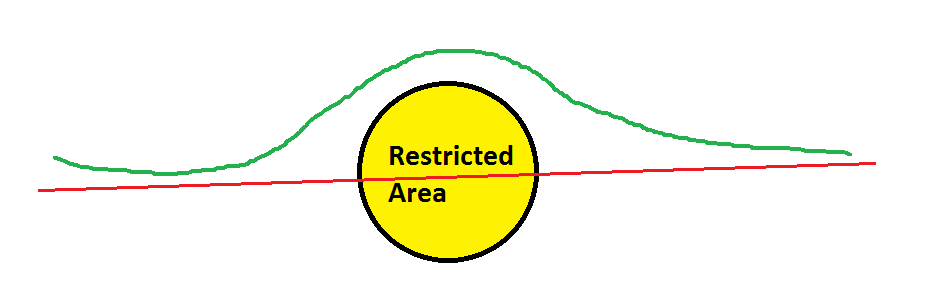
\includegraphics[width=0.7\textwidth]{fig/avoidance.png}
\caption{Not convex avoidance. temporary sketch.}
\label{fig:avoidance}
\end{figure}

For experiment purposes, obstacles will be first approximated with circle and than with half plain. A whole new approach must be applied, because the desired avoidance trajectory might not lie in the allowed space, the great advantage of 


Let's suppose, that the UAV trajectory is a line connecting all predicted positions. If we make sure, that all the positions lie inside the convex space, the whole trajectory has to lie inside a convex space. This is based on the definition of convex space
\begin{equation}
\label{eq:convex_definition}
a,b\in \textbf{M}: \{\lambda a+(1-\lambda) b \mid 0 \leq \lambda \leq 1 \}\in \textbf{M}
\end{equation}
where $\textbf{M}$ is a convex space. 

The linear constrained quadratic programming problem is defined as 


%%  = argmin \frac{1}{2} \textbf{X^T H x} + c^T x

\begin{equation}
\begin{split}
u^\star = arg\ min\ \frac{1}{2} \textbf{u}^T \textbf{Hu}\\
s.\ t. \textbf{A}_c \textbf{u}\leq \textbf{b}_c,\\
\end{split}
\label{eq:quadprog_constrained_definition}
\end{equation}

where $\textbf{A}_c$




\clearpage

% Závěr
\section{Conclusion}

Text text, blah blah, závěr, huhl
\cleardoublepage

% Seznam literatury se nachází v dp.bib
\bibliography{dp}{}
\cleardoublepage
\bibliographystyle{plain}
\clearpage

% Apendixy, schemata, seznam zkratek, atp...
\appendices
\lhead{\emph{APPENDIX \leftmark}} 
\section{CD Content}

In Table~\ref{tab:obsah} are listed names of all root directories on CD.

\vspace{1cm}
\begin{table}[!htb]
\centering
\begin{tabular}{lp{10cm}}
\textbf{Directory name} & \textbf{Description} \\

\hline
thesis & Bachelor's thesis in pdf format.\\
thesis\_sources & latex source codes \\
\hline
\end{tabular}
\caption{CD Content}
\label{tab:obsah}
\end{table}
\cleardoublepage

\section{List of abbreviations}\label{ape:abbreviations}

In Table \ref{table:abbreviations} are listed abbreviations used in this thesis.

\begin{table}[!htb]
\centering
\begin{tabular}{ll}
\textbf{Abbreviation} & \textbf{Meaning} \\
\hline
\textbf{API} & application programming interface \\
\hline
\end{tabular}
\caption{Lists of abbreviations}
\label{table:abbreviations}
\end{table}
\cleardoublepage

\end{document}
